\documentclass[oneside]{book}

\usepackage{amsmath, amsthm, amssymb, amsfonts}
\usepackage{thmtools}
\usepackage{graphicx}
\usepackage{setspace}
\usepackage{geometry}
\usepackage{float}
\usepackage{hyperref}
\usepackage[utf8]{inputenc}
\usepackage[english]{babel}
\usepackage{framed}
\usepackage[dvipsnames]{xcolor}
\usepackage{environ}
\usepackage{tcolorbox}
\tcbuselibrary{theorems,skins,breakable}

\setstretch{1.2}
\geometry{
    textheight=9in,
    textwidth=5.5in,
    top=1in,
    headheight=12pt,
    headsep=25pt,
    footskip=30pt
}

% Variables
\def\notetitle{MATH 165\\Linear Algebra \& Diff. Equation\\Midterm II \\Notes with Examples}
\def\noteauthor{
    \textbf{Professor Kalyani Madhu} \\ 
    % {\LaTeX} 
    by Ethan\\
    University of Rochester}
\def\notedate{Spring 2024}

% The theorem system and user-defined commands
% Theorem System
% The following boxes are provided:
%   Definition:     \defn 
%   Theorem:        \thm 
%   Lemma:          \lem
%   Corollary:      \cor
%   Proposition:    \prop   
%   Claim:          \clm
%   Fact:           \fact
%   Proof:          \pf
%   Example:        \ex
%   Remark:         \rmk (sentence), \rmkb (block)
% Suffix
%   r:              Allow Theorem/Definition to be referenced, e.g. thmr
%   p:              Add a short proof block for Lemma, Corollary, Proposition or Claim, e.g. lemp
%                   For theorems, use \pf for proof blocks

% Definition
\newtcbtheorem[number within=section]{mydefinition}{Definition}
{
    enhanced,
    frame hidden,
    titlerule=0mm,
    toptitle=1mm,
    bottomtitle=1mm,
    fonttitle=\bfseries\large,
    coltitle=black,
    colbacktitle=green!20!white,
    colback=green!10!white,
}{defn}

\NewDocumentCommand{\defn}{m+m}{
    \begin{mydefinition}{#1}{}
        #2
    \end{mydefinition}
}

\NewDocumentCommand{\defnr}{mm+m}{
    \begin{mydefinition}{#1}{#2}
        #3
    \end{mydefinition}
}

% Theorem
\newtcbtheorem[use counter from=mydefinition]{mytheorem}{Theorem}
{
    enhanced,
    frame hidden,
    titlerule=0mm,
    toptitle=1mm,
    bottomtitle=1mm,
    fonttitle=\bfseries\large,
    coltitle=black,
    colbacktitle=cyan!20!white,
    colback=cyan!10!white,
}{thm}

\NewDocumentCommand{\thm}{m+m}{
    \begin{mytheorem}{#1}{}
        #2
    \end{mytheorem}
}

\NewDocumentCommand{\thmr}{mm+m}{
    \begin{mytheorem}{#1}{#2}
        #3
    \end{mytheorem}
}

% Lemma
\newtcbtheorem[use counter from=mydefinition]{mylemma}{Lemma}
{
    enhanced,
    frame hidden,
    titlerule=0mm,
    toptitle=1mm,
    bottomtitle=1mm,
    fonttitle=\bfseries\large,
    coltitle=black,
    colbacktitle=violet!20!white,
    colback=violet!10!white,
}{lem}

\NewDocumentCommand{\lem}{m+m}{
    \begin{mylemma}{#1}{}
        #2
    \end{mylemma}
}

\newenvironment{lempf}{
	{\noindent{\it \textbf{Proof for Lemma}}}
	\tcolorbox[blanker,breakable,left=5mm,parbox=false,
    before upper={\parindent15pt},
    after skip=10pt,
	borderline west={1mm}{0pt}{violet!20!white}]
}{
    \textcolor{violet!20!white}{\hbox{}\nobreak\hfill$\blacksquare$} 
    \endtcolorbox
}

\NewDocumentCommand{\lemp}{m+m+m}{
    \begin{mylemma}{#1}{}
        #2
    \end{mylemma}

    \begin{lempf}
        #3
    \end{lempf}
}

% Corollary
\newtcbtheorem[use counter from=mydefinition]{mycorollary}{Corollary}
{
    enhanced,
    frame hidden,
    titlerule=0mm,
    toptitle=1mm,
    bottomtitle=1mm,
    fonttitle=\bfseries\large,
    coltitle=black,
    colbacktitle=orange!20!white,
    colback=orange!10!white,
}{cor}

\NewDocumentCommand{\cor}{+m}{
    \begin{mycorollary}{}{}
        #1
    \end{mycorollary}
}

\newenvironment{corpf}{
	{\noindent{\it \textbf{Proof for Corollary.}}}
	\tcolorbox[blanker,breakable,left=5mm,parbox=false,
    before upper={\parindent15pt},
    after skip=10pt,
	borderline west={1mm}{0pt}{orange!20!white}]
}{
    \textcolor{orange!20!white}{\hbox{}\nobreak\hfill$\blacksquare$} 
    \endtcolorbox
}

\NewDocumentCommand{\corp}{m+m+m}{
    \begin{mycorollary}{}{}
        #1
    \end{mycorollary}

    \begin{corpf}
        #2
    \end{corpf}
}

% Proposition
\newtcbtheorem[use counter from=mydefinition]{myproposition}{Proposition}
{
    enhanced,
    frame hidden,
    titlerule=0mm,
    toptitle=1mm,
    bottomtitle=1mm,
    fonttitle=\bfseries\large,
    coltitle=black,
    colbacktitle=yellow!30!white,
    colback=yellow!20!white,
}{prop}

\NewDocumentCommand{\prop}{+m}{
    \begin{myproposition}{}{}
        #1
    \end{myproposition}
}

\newenvironment{proppf}{
	{\noindent{\it \textbf{Proof for Proposition.}}}
	\tcolorbox[blanker,breakable,left=5mm,parbox=false,
    before upper={\parindent15pt},
    after skip=10pt,
	borderline west={1mm}{0pt}{yellow!30!white}]
}{
    \textcolor{yellow!30!white}{\hbox{}\nobreak\hfill$\blacksquare$} 
    \endtcolorbox
}

\NewDocumentCommand{\propp}{+m+m}{
    \begin{myproposition}{}{}
        #1
    \end{myproposition}

    \begin{proppf}
        #2
    \end{proppf}
}

% Claim
\newtcbtheorem[use counter from=mydefinition]{myclaim}{Claim}
{
    enhanced,
    frame hidden,
    titlerule=0mm,
    toptitle=1mm,
    bottomtitle=1mm,
    fonttitle=\bfseries\large,
    coltitle=black,
    colbacktitle=pink!30!white,
    colback=pink!20!white,
}{clm}


\NewDocumentCommand{\clm}{m+m}{
    \begin{myclaim*}{#1}{}
        #2
    \end{myclaim*}
}

\newenvironment{clmpf}{
	{\noindent{\it \textbf{Proof for Claim.}}}
	\tcolorbox[blanker,breakable,left=5mm,parbox=false,
    before upper={\parindent15pt},
    after skip=10pt,
	borderline west={1mm}{0pt}{pink!30!white}]
}{
    \textcolor{pink!30!white}{\hbox{}\nobreak\hfill$\blacksquare$} 
    \endtcolorbox
}

\NewDocumentCommand{\clmp}{m+m+m}{
    \begin{myclaim*}{#1}{}
        #2
    \end{myclaim*}

    \begin{clmpf}
        #3
    \end{clmpf}
}

% Fact
\newtcbtheorem[use counter from=mydefinition]{myfact}{Fact}
{
    enhanced,
    frame hidden,
    titlerule=0mm,
    toptitle=1mm,
    bottomtitle=1mm,
    fonttitle=\bfseries\large,
    coltitle=black,
    colbacktitle=purple!20!white,
    colback=purple!10!white,
}{fact}

\NewDocumentCommand{\fact}{+m}{
    \begin{myfact}{}{}
        #1
    \end{myfact}
}


% Proof
\NewDocumentCommand{\pf}{+m}{
    \begin{proof}
        [\noindent\textbf{Proof.}]
        #1
    \end{proof}
}

% Example
\newenvironment{example}{%
    \par
    \vspace{5pt}
	\begin{minipage}{\textwidth}
		\noindent\textbf{Example.}
		\tcolorbox[blanker,breakable,left=5mm,parbox=false,
	    before upper={\parindent15pt},
	    after skip=10pt,
		borderline west={1mm}{0pt}{cyan!10!white}]
}{%
		\endtcolorbox
	\end{minipage}
    \vspace{5pt}
}

\NewDocumentCommand{\ex}{+m}{
    \begin{example}
        #1
    \end{example}
}


% Remark
\NewDocumentCommand{\rmk}{+m}{
    {\it \color{blue!50!white}#1}
}

\newenvironment{remark}{
    \par
    \vspace{5pt}
    \begin{minipage}{\textwidth}
        {\par\noindent{\textbf{Remark.}}}
        \tcolorbox[blanker,breakable,left=5mm,
        before skip=10pt,after skip=10pt,
        borderline west={1mm}{0pt}{cyan!10!white}]
}{
        \endtcolorbox
    \end{minipage}
    \vspace{5pt}
}

\NewDocumentCommand{\rmkb}{+m}{
    \begin{remark}
        #1
    \end{remark}
}


\newcommand{\lcm}{\operatorname{lcm}}



% ------------------------------------------------------------------------------

\begin{document}
\title{\textbf{
    \LARGE{\notetitle} \vspace*{10\baselineskip}}
    }
\author{\noteauthor}
\date{\notedate}

\maketitle
\newpage

\tableofcontents
\newpage

% ------------------------------------------------------------------------------







\chapter{Determinants}
\section{Lecture 9: Def. of Determinants \& it's calculation}

\rmk{
    This lecture covers: 
    % \\ - 3.1 The Definition of the Determinant\\- 3.3 Cofactor Expansions (partly)
    \begin{itemize}
        \item 3.1 The Definition of the Determinant
        \item 3.3 Cofactor Expansions (partly)
    \end{itemize}
}

\subsection{What is Determinanrts}

\defn{Determinants}{
    The \textbf{determinants} of a square matrix $A$, denoted $\det{(A)}$, is a number associated with the matrix $A$ that is \textit{designed} to carry information about the invertibility (among other things) of the matrix $A$. We also use the notation $|A|$ to denote the determinant of $A$. 
}
The way we calculate determinants is derived from the fact of changing the matrix into RREF (Reduce-Row-Echelon-Form) and seeing if the matrix is invertible. If the matrix is invertible, then the determinant is not zero. If the matrix is not invertible, then the determinant is zero. The way we calculate it is based on observation. (P.196)

\subsection{How to calculate Determinants}
\paragraph{1 by 1 matrix}

The determinant of a $1 \times 1$ matrix $[a11]$ is $a_{11}$. 

\ex{
    \\
    \textbf{Calculate the determinant of the matrix $A = [3]$. }
    \[
        \begin{vmatrix}
            3
        \end{vmatrix} = 3
    \]
    \textbf{What is the rank of the matrix $A$? } \\The rank of the matrix $A$ is 1.

}
\\\\
\ex{
    \\
    \textbf{Calculate the determinant of the matrix $A = [0]$. }\\
    \[
        \begin{vmatrix}
            0
        \end{vmatrix} = 0
    \]
    \textbf{What is the rank of the matrix $A$? } \\
    The rank of the matrix $A$ is 0. (Since the determinant is 0, the matrix is not invertible.)

}


\paragraph{2 by 2 matrix} 

The determinant of a $2 \times 2$ matrix $A = \begin{bmatrix} a & b \\ c & d \end{bmatrix}$ is given by $ad=bc$. 
\[
    \begin{vmatrix}
        a & b \\
        c & d
    \end{vmatrix} 
    = ad - bc
\]

The way we calculate it is by taking the product of the diagonal elements and subtracting the product of the off-diagonal elements.


\ex{
    \textbf{Calculate the determinant of the matrix $A = \begin{bmatrix} 1 & 2 \\ 3 & 4 \end{bmatrix}$. }
    \[
        \begin{vmatrix}
            1 & 2 \\
            3 & 4
        \end{vmatrix} = 1 \cdot 4 - 2 \cdot 3 = 4 - 6 = -2
    \]
    \textbf{What is the rank of the matrix $A$? } \\The rank of the matrix $A$ is 2.\\
    \textbf{Is the matrix invertible? } \\Yes, the matrix is invertible, since $-2 \neq 0$.
}

\ex{
    \textbf{Calculate the determinant of the matrix $A = \begin{bmatrix} 2 & 3 \\ 4 & 6 \end{bmatrix}$. }
    \[
        \begin{vmatrix}
            2 & 3 \\
            4 & 6
        \end{vmatrix} = 2 \cdot 6 - 3 \cdot 4 = 12 - 12 = 0
    \]
    \textbf{What is the rank of the matrix $A$? } \\The rank of the matrix $A$ is 1.\\
    \textbf{Is the matrix invertible? } \\No, the matrix is not invertible, since $0 = 0$.
}



\paragraph{3 by 3 matrix}
The determinant of a $ 3 \times 3 $ matrixhas a similar 'diagonals'-type definition:
\[
    |A|= \begin{vmatrix}
        a & b & c \\
        d & e & f \\
        g & h & i
    \end{vmatrix}
    = aei + bfg + cdh - ceg - bdi - afh
\]


We can use a clever trick with arrows by repeating the first two columns to calculate the determinant of a $3 \times 3$ matrix.



\begin{figure}
    \begin{center}
        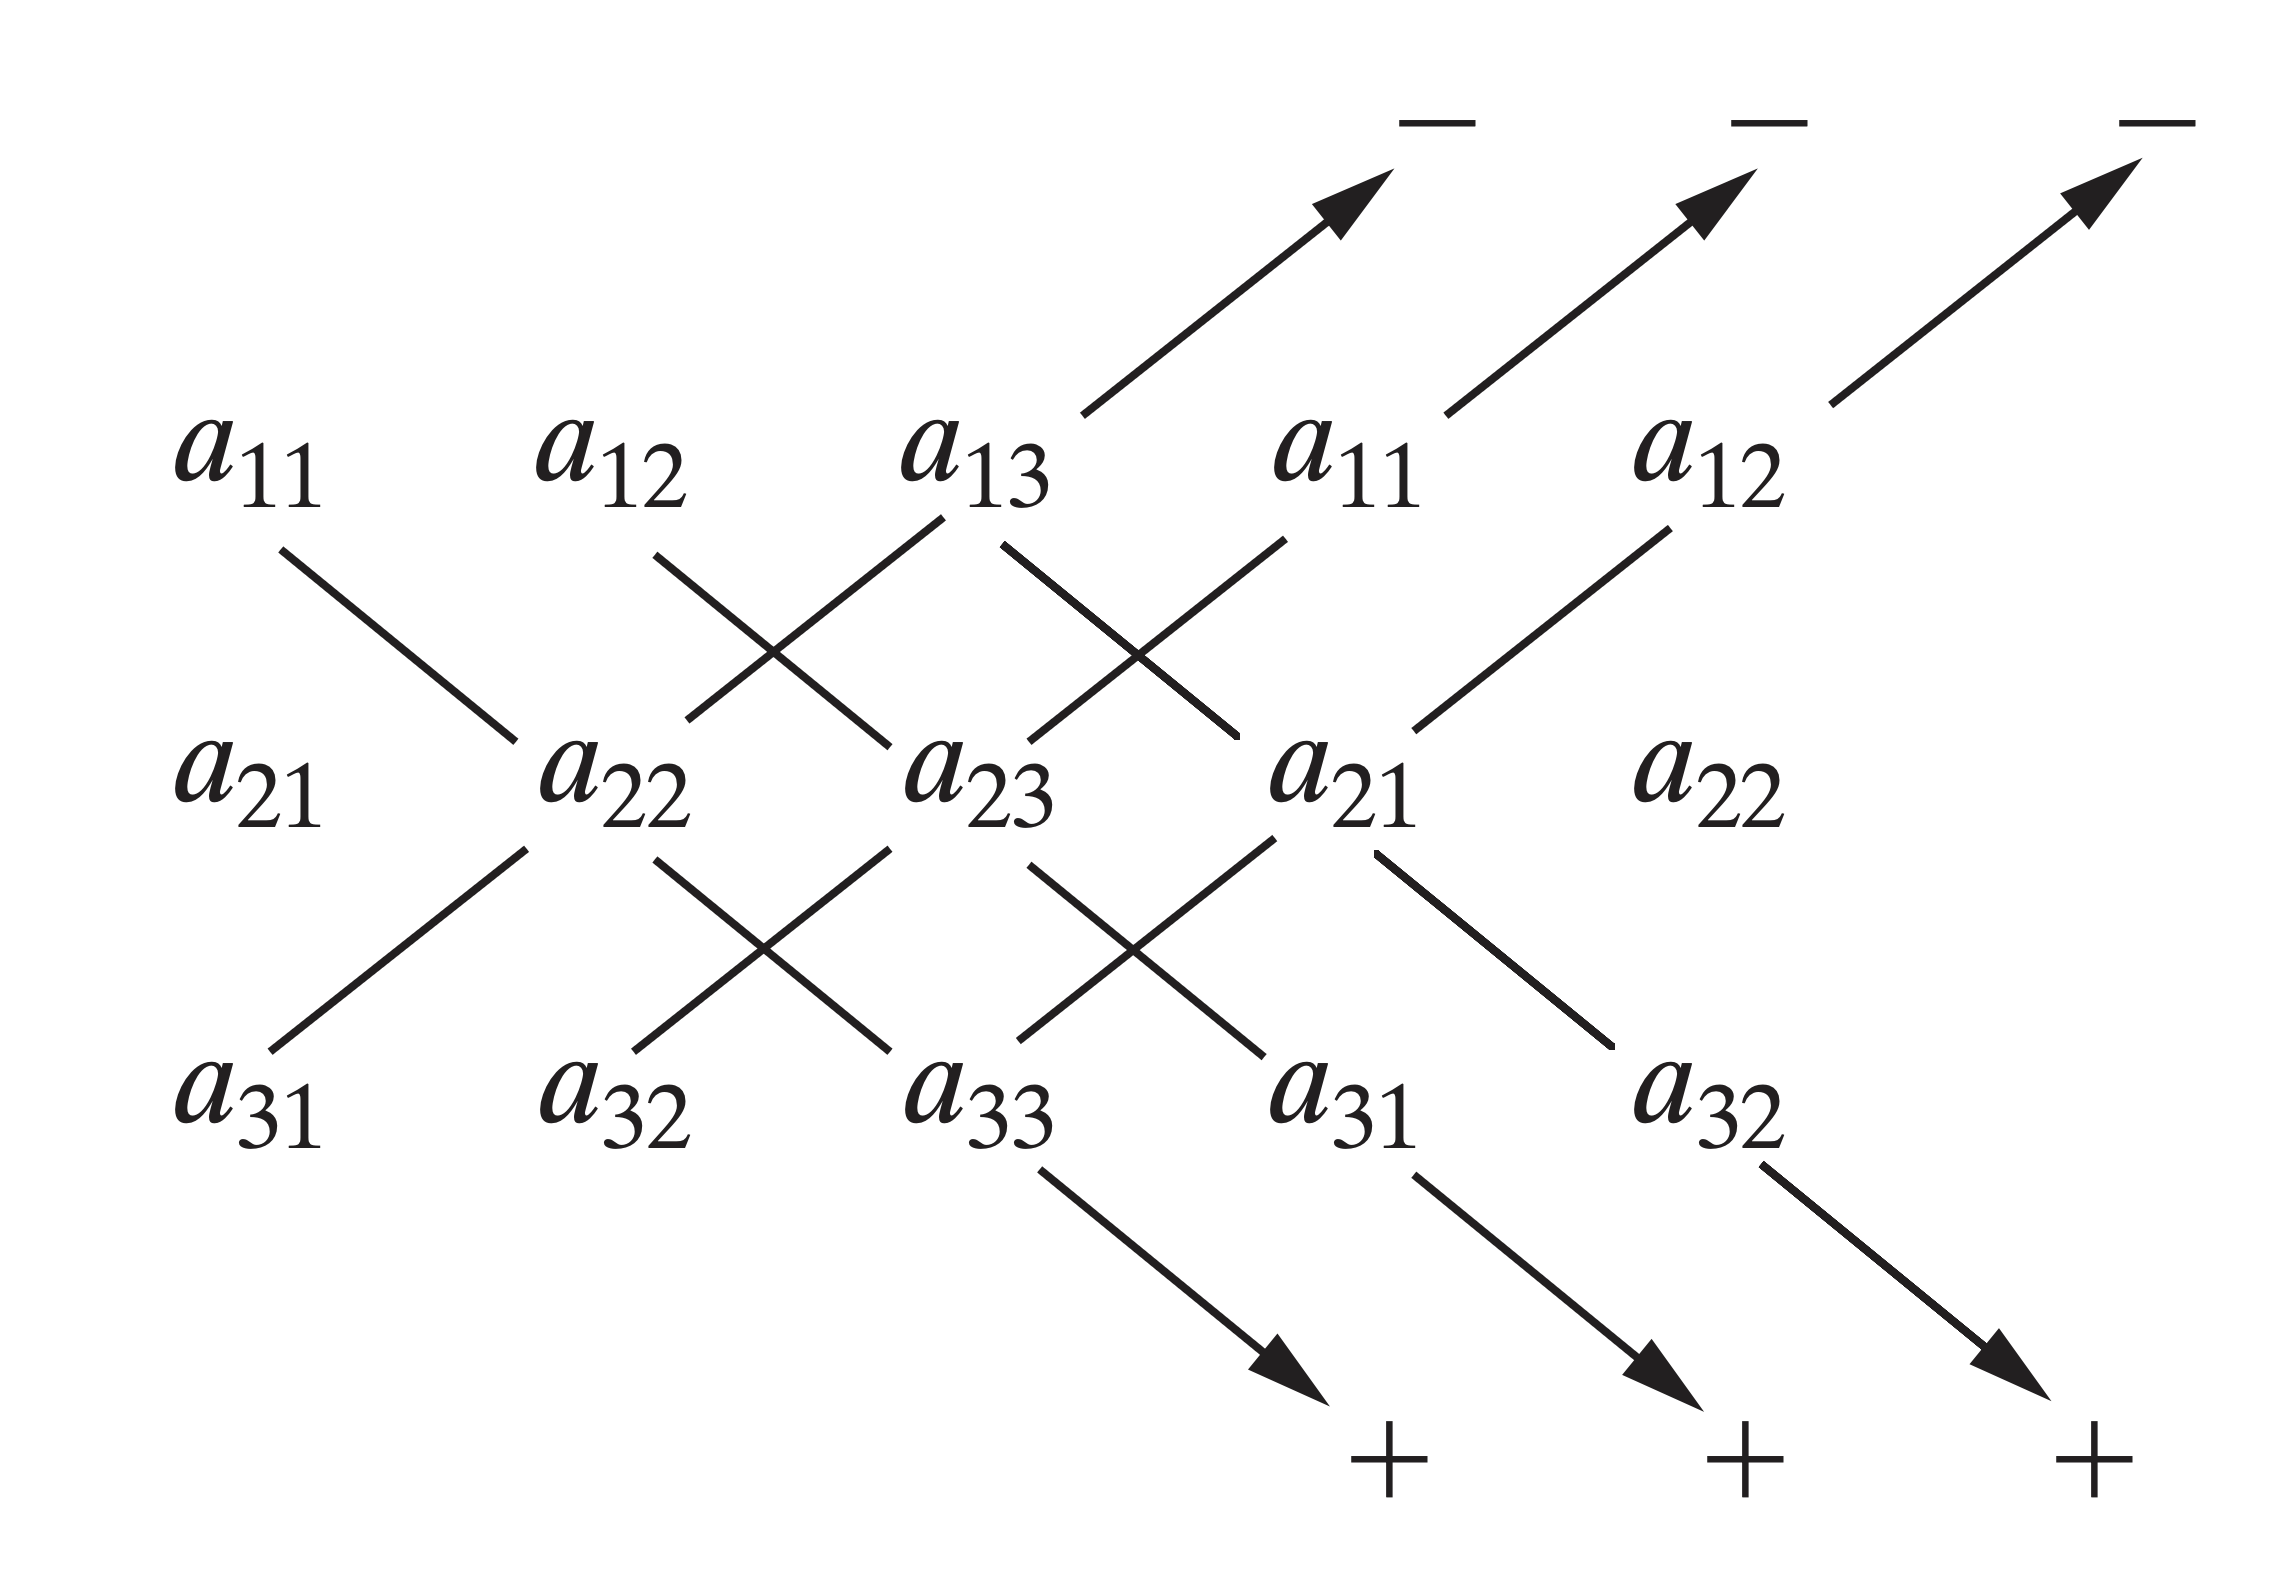
\includegraphics[scale=0.1]{img/Snipaste_2024-03-27_13-52-06.png}
        \caption{Determinant of a $3 \times 3$ matrix}
    \end{center}
\end{figure}





\ex{
    \textbf{Calculate the determinant of the matrix $A = \begin{bmatrix} 1 & 2 & 3 \\ 4 & 5 & 6 \\ 7 & 8 & 9 \end{bmatrix}$. }
    \[
        \begin{vmatrix}
            1 & 2 & 3 \\
            4 & 5 & 6 \\
            7 & 8 & 9
        \end{vmatrix} = 1 \cdot 5 \cdot 9 + 2 \cdot 6 \cdot 7 + 3 \cdot 4 \cdot 8 - 3 \cdot 5 \cdot 7 - 2 \cdot 4 \cdot 9 - 1 \cdot 6 \cdot 8 = 0
    \]
    \textbf{What is the rank of the matrix $A$? } \\The rank of the matrix $A$ is 2.\\
    \textbf{Is the matrix invertible? } \\No, the matrix is not invertible, since $0 = 0$.

}


\rmkb{
    If the dimension of a matrix is greater than $3 \times 3$, we won’t be able to find the determinant in one step, as the sub-matrices will have dimension at least $3 \times 3$.
}


\paragraph{Larger matrix}

Another more common way to find the determinant of a $3 \times 3$ matrix is to use the \textbf{cofactor expansion} method. The cofactor expansion method is a way to calculate the determinant of a matrix by breaking it down into smaller matrices. This can also apply to \textbf{larger matrices}.
\[
    \begin{vmatrix}
        a & b & c \\
        d & e & f \\
        g & h & i
    \end{vmatrix} 
    = a \begin{vmatrix}
        e & f \\
        h & i
    \end{vmatrix} - b \begin{vmatrix}
        d & f \\
        g & i
    \end{vmatrix} + c \begin{vmatrix}
        d & e \\
        g & h
    \end{vmatrix}
\]

\thmr{Cofactor Expansion}{}{
    We may expand along row $i$:

    \[
        \det(A) = a_{i1}C_{i1} + a_{i2}C_{i2} + \cdots + a_{in}C_{in} = \sum_{j=1}^{n} a_{ij}C_{ij}
    \]


    We may expand along column $j$:

    \[
        \det(A) = a_{1j}C_{1j} + a_{2j}C_{2j} + \cdots + a_{nj}C_{nj} = \sum_{i=1}^{n} a_{ij}C_{ij}
    \]

}


The way you do so is to choose a row or a column (typically, a row or column with the most zeros) and expand the determinant along that row or column. If the matrix after expansion is still not a $2 \times 2$ matrix, you can expand it again.



\ex{\\
    \textbf{Calculate the determinant of the matrix $A = \begin{bmatrix} 1 & 2 & 3 & 4 \\ 5 & 6 & 7 & 8 \\ 9 & 10 & 11 & 12 \\ 13 & 14 & 15 & 16 \end{bmatrix}$. }\\\\\\
    Let's choose the first row to expand the determinant.
    \[
        \begin{vmatrix}
            1 & 2 & 3 & 4 \\
            5 & 6 & 7 & 8 \\
            9 & 10 & 11 & 12 \\
            13 & 14 & 15 & 16
        \end{vmatrix} 
        = 1 \begin{vmatrix}
            6 & 7 & 8 \\
            10 & 11 & 12 \\
            14 & 15 & 16
        \end{vmatrix} - 2 \begin{vmatrix}
            5 & 7 & 8 \\
            9 & 11 & 12 \\
            13 & 15 & 16
        \end{vmatrix} + 3 \begin{vmatrix}
            5 & 6 & 8 \\
            9 & 10 & 12 \\
            13 & 14 & 16
        \end{vmatrix} - 4 \begin{vmatrix}
            5 & 6 & 7 \\
            9 & 10 & 11 \\
            13 & 14 & 15
        \end{vmatrix}
    \]
    % \\\\\\\\\\\\
    \[
        = 1 \times 6 \begin{vmatrix}
            11 & 12 \\
            15 & 16
        \end{vmatrix} - 2 \times 7 \begin{vmatrix}
            9 & 12 \\
            13 & 16
        \end{vmatrix} + 3 \times 8 \begin{vmatrix}
            9 & 11 \\
            13 & 15
        \end{vmatrix} - 4 \times 5 \begin{vmatrix}
            10 & 11 \\
            14 & 15
        \end{vmatrix} \text{...} = 0
    \]
    \\
    \textbf{What is the rank of the matrix $A$? } \\The rank of the matrix $A$ is 2.\\\\
    \textbf{Is the matrix invertible? } \\No, the matrix is not invertible, since $0 = 0$.\\
}

\subsection{Inverse of 2 by 2 matrix}

\prop{
    Let $A = \begin{bmatrix} a & b \\ c & d \end{bmatrix}$ be a $2 \times 2$ matrix. If $\det(A) \neq 0$, then the inverse of $A$ is given by
    \[
        A^{-1} = \frac{1}{\det(A)} \begin{bmatrix} d & -b \\ -c & a \end{bmatrix}
    \]

}
\pf{
    Let $A = \begin{bmatrix} a & b \\ c & d \end{bmatrix}$ be a $2 \times 2$ matrix. If $\det(A) \neq 0$, then
    \[
        A = \begin{pmatrix}
        a & b \\
        c & d
    \end{pmatrix}
    \]
    \[
        A^{-1} = \frac{1}{\det(A)} \begin{bmatrix} d & -b \\ -c & a \end{bmatrix}
    \]
    \[
        = \frac{1}{ad - bc} \begin{bmatrix} d & -b \\ -c & a \end{bmatrix}
    \]
    \[
        A \times A^{-1} = \begin{pmatrix}
        a & b \\
        c & d
        \end{pmatrix} \times \frac{1}{ad - bc} \begin{pmatrix}
        d & -b \\
        -c & a
        \end{pmatrix}
    \]
    \[
        \frac{1}{ad - bc}(a \times d + b \times (-c)) = \frac{ad - bc}{ad - bc} = 1
    \]
    \[
        \frac{1}{ad - bc}(a \times (-b) + b \times a) = \frac{-ab + ab}{ad - bc} = 0
    \]
    \[
        \frac{1}{ad - bc}(c \times d + d \times (-c)) = \frac{cd - cd}{ad - bc} = 0
    \]
    \[
        \frac{1}{ad - bc}(c \times (-b) + d \times a) = \frac{-bc + ad}{ad - bc} = 1
    \]
    \[
        A \times A^{-1}
        =
        \begin{pmatrix}
            1 & 0 \\
            0 & 1
        \end{pmatrix}
        = I
    \]

    Thus, $A^{-1} = \frac{1}{\det(A)} \begin{bmatrix} d & -b \\ -c & a \end{bmatrix}$.

}

\ex{
    \textbf{Find the inverse of the matrix $A = \begin{bmatrix} 1 & 2 \\ 3 & 4 \end{bmatrix}$. }
    \[
        \begin{vmatrix}
            1 & 2 \\
            3 & 4
        \end{vmatrix} = 1 \cdot 4 - 2 \cdot 3 = 4 - 6 = -2
    \]
    Since $\det(A) = -2 \neq 0$, we can find the inverse of $A$.
    \[
        A^{-1} = \frac{1}{-2} \begin{bmatrix} 4 & -2 \\ -3 & 1 \end{bmatrix} = \begin{bmatrix} -2 & 1 \\ 3/2 & -1/2 \end{bmatrix}
    \]

}




\subsection{Determinat of matrix functions}
Given a matrix function $M (t)$, its determinant $\det(M (t))$ can be found using exactly the same techniques as that of a numerical matrix. The only difference is that the determinant is a function of t.

\ex{
    \textbf{Find} \[
        \begin{vmatrix}
            \cos(t) & -\sin(t) \\
            \cos(t) & \sin(t)
        \end{vmatrix}
    \]

    \[
        \begin{vmatrix}
            \cos(t) & -\sin(t) \\
            \cos(t) & \sin(t)
        \end{vmatrix}
        = \cos(t) \cdot \sin(t) - (-\sin(t) \cdot \cos(t))
    \]
    \[
        = \sin(t) \cdot \cos(t) + \sin(t) \cdot \cos(t) 
    \]
    \[= 2 \sin(t) \cdot \cos(t)\]
    \[\boxed{= \sin(2t)} \]

}





\subsection{Geometry Application: areas and volumes}

\paragraph{Areas}
Suppose $O$ is the origin in the xy-plane. Let P be a parallelogram with vertices $O = (0, 0)$,$ A = (a_1, a_2)$, $B = (b_1, b_2)$, and $C = (c_1, c_2)$.

\fact{
    The area of the parallelogram P is given by
    \[
        \text{Area}(P) = \begin{vmatrix}
            \det \begin{pmatrix}
                \begin{bmatrix}
                    a_1 & a_2 \\
                    b_1 & b_2
                \end{bmatrix}
            \end{pmatrix}
        \end{vmatrix}
    \]
}
Since the area is always positive, we take the absolute value of the determinant.


\paragraph{Volumes}
Similarly, the volume of a parallelepiped in $\mathbb{R}^3$ is given by the absolute value of the determinant of the matrix whose rows are the vectors representing the edges of the parallelepiped.

\fact{
    The volume of the parallelepiped determined by sides $OA$, $OB$, and $OC$ where
    \[
        A=(a_1, a_2, a_3), B=(b_1, b_2, b_3), C=(c_1, c_2, c_3)
    \]
    is given by
    \[
        \text{Volume} = \begin{vmatrix}
            \det \begin{pmatrix}
                \begin{bmatrix}
                    a_1 & a_2 & a_3 \\
                    b_1 & b_2 & b_3 \\
                    c_1 & c_2 & c_3
                \end{bmatrix}
            \end{pmatrix}
        \end{vmatrix}
    \]

}


\pf{
    The area of the parallelogram is 
    Area = (length of base) $\times$ (perpendicular height).\\
    This can be written as \\
    \[
        \text{Area } = ||a||h = ||a||  ||b|| \space \sin(\theta) ||a \times b||
    \]
    Since the k components of a and b are both zero (since the vectors lie in thexy-plane), substitution from Equation yields
    \[
        \text{Area} = ||(a_1 b_2 - a_2 b_1)k|| = |a_1 b_2 - a_2 b_1| = |\det(A)|.
    \]
}

\begin{figure}
    \begin{center}
        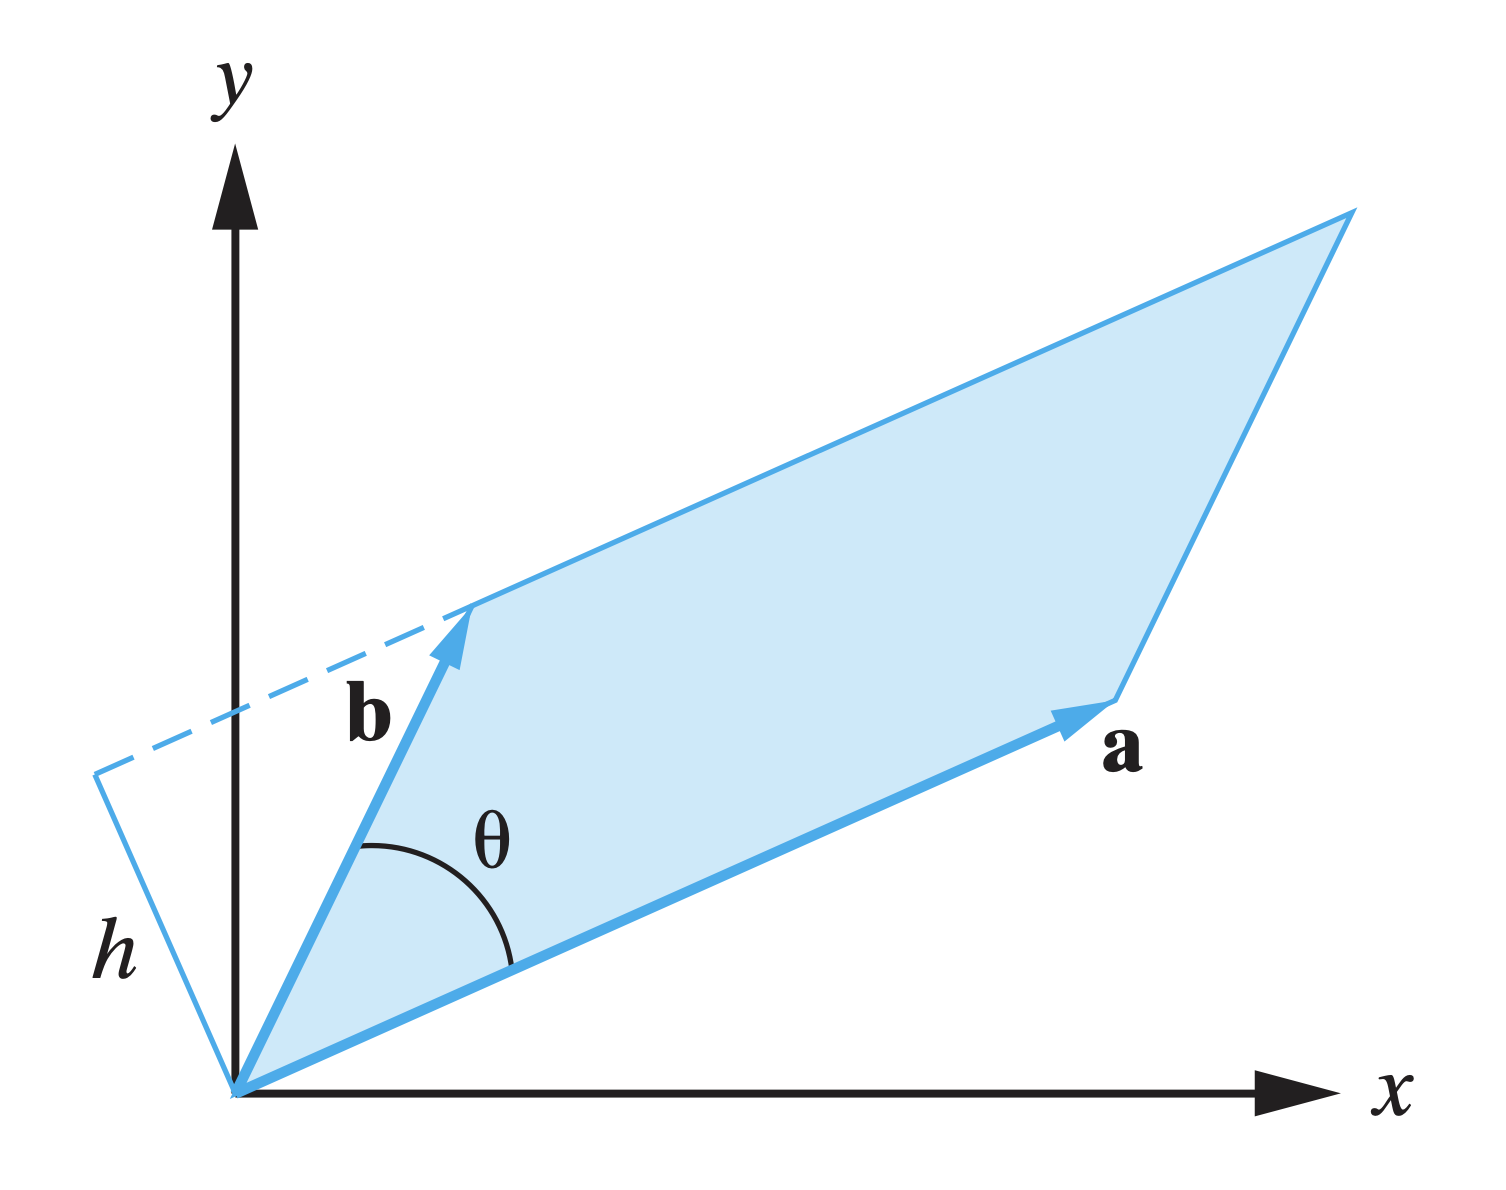
\includegraphics[scale=0.2]{img/Snipaste_2024-03-27_22-33-20.png}
        \caption{Area of a parallelogram}    
    \end{center}
\end{figure}




\ex{
    \textbf{Find the area of the triangle with vertices $(1,1), (2,3), (6,9)$.}
    \[
        \begin{vmatrix}
            1 & 1 \\
            2 & 3
        \end{vmatrix}
        = 1 \cdot 3 - 1 \cdot 2 = 3 - 2 = \boxed{1}
    \]
    Note: Since the vector $(6, 9)$ is a multiple of the vector $(2, 3)$ (linearly dependent), we can ignore the third vertex $(6, 9)$.

    



}


\newpage
% ------------------------------------------------------------------------------
\section{Lecture 10: Rank, Invertibility, Elementary Row Operations \& additional properties of determinants}
\rmk{
    This lecture covers: 
    \begin{itemize}
        \item 3.2 Properties of Determinants
    \end{itemize}
}




\subsection{Determinants, Rank, Invertibility}

\thmr{}{}{
    Let $A$ be an upper (or lower) triangular square matrix. Then $\det(A)$ is the product of the diagonal entries of $A$.
}

\pf{
    Let $A$ be an upper triangular matrix. Then $A$ can be written as
    \[
        A = \begin{bmatrix}
            a_{11} & a_{12} & \cdots & a_{1n} \\
            0 & a_{22} & \cdots & a_{2n} \\
            \vdots & \vdots & \ddots & \vdots \\
            0 & 0 & \cdots & a_{nn}
        \end{bmatrix}
    \]
    Then
    \[
        \det(A) = a_{11} \begin{vmatrix}
            a_{22} & \cdots & a_{2n} \\
            \vdots & \ddots & \vdots \\
            0 & \cdots & a_{nn}
        \end{vmatrix}
        = a_{11} \cdot a_{22} \cdots a_{nn}
    \]

}

Since the possible effect on the determinant of putting a matrix into row-echelon form can only be multiplied by a non-zero constant, for an $n \times n$ matrix $A$, $\det(A) = 0$ if and only if the product of the diagonal entries of a row-echelon form of $A$ is zero. This happens if and only if the rank of $A$ is less than $n$.
\\


\ex{
    \textbf{Calculate the determinant of the matrix $A = \begin{bmatrix} 1 & 2 & 3 \\ 0 & 4 & 5 \\ 0 & 0 & 6 \end{bmatrix}$. }
    \[
        \begin{vmatrix}
            1 & 2 & 3 \\
            0 & 4 & 5 \\
            0 & 0 & 6
        \end{vmatrix} = 1 \cdot 4 \cdot 6 = 24
    \]
    \textbf{What is the rank of the matrix $A$? } \\The rank of the matrix $A$ is 3.\\
    \textbf{Is the matrix invertible? } \\Yes, the matrix is invertible, since $24 \neq 0$.
}

The following theorem is based on the previous theorem.

\rmkb{
    \textbf{Rank} is the number of linearly independent rows (or columns) of a matrix, which is also equal to the number of leading 1's in the RREF of the matrix.
}
\thmr{}{Theorem 3.2.1}{
    Let $A$ be an $n \times n$ matrix. Then $\det(A) \neq 0$ if and only if rank($A$) = $n$.\\
}

This means that whether or not a square matrix $A$ has a non-zero determinant tells us whether or not $A$ is invertible and whether or not $Ax=0$ has a unique solution.

\ex{
    \textbf{Let $A = \begin{bmatrix} 5 & 9 & 6 \\ 0 & 3 & 7 \\ 0 & 0 & 8 \end{bmatrix}$. Find the rank of $A$. } \\
    \[ 
        \det(A) = 5 \dots 3 \dots 8 = 120 \neq 0
    \]
    Since $\det(A) \neq 0$, $A$ is a $3 \times 3$ matrix,the rank of $A$ is 3.\\
}   




Since it’s easy to find the determinant of row-echelon matrices, and also as a step to proving Thm. 3.2.5, we are interested in the effect of EROs on determinants.


\subsection{Elementary Row Operations}


\thmr{}{}{
    \textbf{Multiplying} a row of a matrix by a scalar $k$ multiplies the determinant of the matrix by $k$.
}

Let $A  = \begin{bmatrix}
    a & b & c\\
    d & e & f\\
    g & h & i
\end{bmatrix}$ and $B = \begin{bmatrix}
    a & b & c\\
    kd & ke & kf\\
    g & h & i
\end{bmatrix}$. \\
Then 
\\
\[
    \mid A \mid = -d \begin{vmatrix}
        b & c\\
        h & i
    \end{vmatrix} + e \begin{vmatrix}
        a & c\\
        g & i
    \end{vmatrix} - f \begin{vmatrix}
        a & b\\
        g & h
    \end{vmatrix}
\]

\[
    \mid B \mid = -kd \begin{vmatrix}
        b & c\\
        h & i
    \end{vmatrix} + ke \begin{vmatrix}
        a & c\\
        g & i
    \end{vmatrix} - kf \begin{vmatrix}
        a & b\\
        g & h
    \end{vmatrix}
\]\\

Therefore, $\mid B \mid = k \mid A \mid$.\\
\newpage
\ex{\\
    Find $\begin{vmatrix}
        1 & 0 & 1\\
        2 & 4 & 2\\
        0 & -1 & -1
    \end{vmatrix}$
    by "factoring" a 2 from the second row. 
    \[
        \begin{vmatrix}
            1 & 0 & 1\\
            2 & 4 & 2\\
            0 & -1 & -1
        \end{vmatrix} = 
        2
        \begin{vmatrix}
            1 & 0 & 1\\
            1 & 2 & 1\\
            0 & -1 & -1
        \end{vmatrix}
    \]
    \[
        = 2 \times 
        \begin{pmatrix}
            2 \begin{vmatrix}
                2 & 1\\
                -1 & -1
            \end{vmatrix} + 1 \begin{vmatrix}
                1 & 2\\
                0 & -1
            \end{vmatrix}
        \end{pmatrix}
    \]
    \[
        = 2 \times (2 \cdot (-2 - (-1)) + 1 \cdot (-1 - 0)) = 2 \times (-2) = \boxed{-4}
    \]

}

Note: Since we are multiplying the entire matrix by the scalar, we are actually raising each row by the scalar. Therefore, the determinant of the matrix should be raised by the scalar to the power of the number of rows.  
\cor{
    If $A$ is a square matrix, then $\det(kA) = k^n \det(A)$.
}


\ex{
    Suppose $A$ is a $4 \times 4$ metaix and $\det(A) = 3 $. What is the determinant of $2A$?
    \[
        \det(2A) = 2^4 \det(A) = 16 \cdot 3 = \boxed{48}
    \]
}



\thmr{}{}{
    \textbf{Exchanging} two rows of a matrix changes the sign of the determinant of the matrix.
}
\ex{\\
    Find $\begin{vmatrix}
        0 & b & 0\\
        a & 0 & 0\\
        0 & 0 & c
    \end{vmatrix}$\\

    \[
        \begin{vmatrix}
            0 & b & 0\\
            a & 0 & 0\\
            0 & 0 & c
        \end{vmatrix} = - \begin{vmatrix}
            a & 0 & 0\\
            0 & b & 0\\
            0 & 0 & c
        \end{vmatrix} =\boxed{-abc}
    \]

}

\thmr{}{}{
    \textbf{Adding} a multiple of one row to another row \textbf{does not change the determinant} of the matrix.
}


\ex{\\
    Find $\begin{vmatrix}
        a+2c & b+2d\\
        c & d
    \end{vmatrix}$
    \[
        \begin{vmatrix}
            a+2c & b+2d\\
            c & d
        \end{vmatrix} 
        \overset{R_1-2R_2}{\longrightarrow} \begin{vmatrix}
            a & b\\
            c & d
        \end{vmatrix}
        = \boxed{ad - bc}
    \]
    
}



\subsection{Additional Properties of Determinants}
\prop{
    If 
    $C = \begin{bmatrix}
        r_1\\
        \vdots\\
        r_{i-1}\\
        a + b \\
        r_{i+1}\\
        \vdots\\
        r_n
    \end{bmatrix}$
    , and 
    $A = \begin{bmatrix}
        r_1\\
        \vdots\\
        r_{i-1}\\
        a \\
        r_{i+1}\\
        \vdots\\
        r_n
    \end{bmatrix}$
    , and
    $B = \begin{bmatrix}
        r_1\\
        \vdots\\
        r_{i-1}\\
        b \\
        r_{i+1}\\
        \vdots\\
        r_n
    \end{bmatrix}$
    , then 
    $\det(C) = \det(A) + \det(B)$.
        
}

\rmkb{
    This property does \textbf{NOT} mean $\det(A+B) = \det(A) + \det(B)$
}

\ex{
    Let $A = \begin{bmatrix}
        2 & 4\\
        -1 & 0
    \end{bmatrix}, B = \begin{bmatrix}
        1 & -1\\
        -1 & 0
    \end{bmatrix}, C = \begin{bmatrix}
        3 & 3\\
        -1 & 0
    \end{bmatrix}$. Find the determinant of these three matrices and relate them to the property.
    \[
        \det(A) = 2 \cdot 0 - 4 \cdot (-1) = \boxed{4}
    \]
    \[
        \det(B) = 1 \cdot 0 - (-1) \cdot (-1) = \boxed{-1}
    \]
    \[
        \det(C) = 3 \cdot 0 - 3 \cdot (-1) = \boxed{3}
    \]
    Notice that the second column of these three matrix are the same. Therefore, we can use the property to find the determinant of $C$. 
    \[
        \det(C) = \det(A) + \det(B) = 4 + -1 = \boxed{3}
    \]
}

\prop{
    If $A$ is a square matrix, then $\det(A^T) = \det(A)$.
}
\pf{
    Let $A = \begin{bmatrix}
        a & b\\
        c & d
    \end{bmatrix}$. Then $A^T = \begin{bmatrix}
        a & c\\
        b & d
    \end{bmatrix}$. Then $\det(A) = ad - bc$ and $\det(A^T) = ad - bc$. Therefore, $\det(A) = \det(A^T)$.
}

\prop{
    The effects on the determinant of elementary row operations still hold when the word row is replaced by the word column. 
}

\prop{
    Since the rank of a square $n \times n$ matrix is n if and only if the determinant is non-zero,
\begin{itemize}
    \item If a matrix has a row (or column) of zeros, then it has determinant zero.
    \item If a matrix has two identical rows (or columns), then it has determinant zero.
    \item If a row (or column) of a matrix is a multiple of another, then it has determinant zero.
\end{itemize}
}


\prop{
    Determinet is multiplicative. That is, if $A$ and $B$ are square matrices of the same size, then $\det(AB) = \det(A) \det(B)$.
}
To get an idea of why this might be true, suppose A and B are upper-triangular matrices. Then AB is also upper-triangular.

\ex{
    \textbf{Let $A = \begin{bmatrix}
        a & b\\
        0 & c
    \end{bmatrix}$
    and $B = \begin{bmatrix}
        d & e\\
        0 & f
    \end{bmatrix}$. Find $\det(AB)$ and $\det(A) \det(B)$.}
    \[
        \det(AB) = \det \begin{pmatrix}
            a \cdot d + b \cdot 0 & a \cdot e + b \cdot f\\
            0 \cdot d + c \cdot 0 & 0 \cdot e + c \cdot f
        \end{pmatrix} = \det \begin{pmatrix}
            ad & ae + bf\\
            0 & cf
        \end{pmatrix} = ad \cdot cf = \boxed{acdf}
    \]
    \textbf{Why can we extend this to non-upper-triangular matrices?} \\
    By changing the order of the rows and columns of a matrix, we can put it into an upper-triangular form without changing the determinant. This is because we can do that only by adding a row to another without multiplication and switching rows. Therefore, we can make the $\det$ stay the same.


    
}

\textbf{If the determinant is multiplicative, what can we say about $\det(A^{-1})$?
}

Let $\det(A) = k$. 
\[
    \det(A) \det(A^{-1}) = \det(AA^{-1}) = \det(I) = 1
\]
\[
    \det(A^{-1}) = \frac{1}{k}
\]




\subsection{More about Determinants}


Relationship between the determinant and the invertibility of a matrix:
\[
    \det(A) = 0 \iff \text{A is not invertible}
\]
\[
    \det(A) \neq 0 \iff \text{A is invertible}
\]
\\
Relationship between the determinant, rank, and number of solutions of a system of linear equations:
\[
    \det(A) = 0 \iff \text{rank}(A) < n \iff \text{system has infinitely many solutions}
\]
\[
    \det(A) \neq 0 \iff \text{rank}(A) = n \iff \text{system has a unique solution}
\]

\ex{
    \textbf{Determine all values of $k$ for which the given system has an infinite number of solutions.}
    \[
        \begin{matrix}
            x_1 +2x_2 + kx_3 & = & 0\\
            2x_1 -kx_2 + x_3 & = & 0\\
            3x_1 + 6x_2 + x_3 & = & 0
        \end{matrix}
    \]
    Approach 1: Use detrerminant:\\
    Let
    \[
        \begin{vmatrix}
            1 & 2 & k\\
            2 & -k & 1\\
            3 & 6 & 1
        \end{vmatrix} = 0
    \]\\
    If $\det(A) \neq 0 $ the rank $\neq n$. Because the system is homogeneous $(Ax=0)$, we don't need to worry about consistency (It is always consistent), therefore, the system has an infinite number of solutions. \\
    \[
        \det(A) = 1 \begin{vmatrix}
            -k & 1\\
            6 & 1
        \end{vmatrix} - 2 \begin{vmatrix}
            2 & 1\\
            3 & 1
        \end{vmatrix} + k \begin{vmatrix}
            2 & -k\\
            3 & 6
        \end{vmatrix} = 0
    \]
    \[
        = -k - 6 - 2(2-3) + k(12 +3k)= 0
    \]
    \[
        -k -6 +2 + 12k +3 k^2 = 0
    \]
    \[
        (3k-1)(k+4)=0
    \]
    \[
        k_1 = \boxed{\frac{1}{3}}, \space
        k_2 = \boxed{-4}
    \]
    Approach 2: Use rank:\\
    \[
        \begin{bmatrix}
            1 & 2 & k & 0\\
            2 & -k & 1 & 0\\
            3 & 6 & 1 & 0
        \end{bmatrix}
    \]
    Row reduce: \\
    \[
        \begin{bmatrix}
            \begin{array}{ccc|c}
                1 & 2 & k & 0\\
                0 & \textbf{-4-k} & 1-2k & 0\\
                0 & 0 & \textbf{1-3k} & 0
            \end{array}
        \end{bmatrix}
    \]
    We can notice that if $1-3k = 0$, the matrix will have at most 2 pivots since the rank is 0. \\
    if $-4-k = 0$, $k = -4$, we can clear the second row to get the third row. Therefore, the system has an infinite number of solutions:\\ 
    \[
        \begin{bmatrix}
            \begin{array}{ccc|c}
                1& 2 & k & 0\\
                0 & \textbf{0}& 1-2k & 0\\
                0 & 0 & 1-3k & 0
            \end{array}
        \end{bmatrix}
    \]
    These two approaches give us the same result. 

}
\\ 
However, the example matrix above will only work if the matrix is homogeneous.  \\

This is because, in a homogeneous system, the rank $A$ will always equal to rank $A^{\#}$ (the augmented matrix)and the system is always consistent.\\

But if not homogeneous, we need to check the consistency of the system. If the rank of $A$ is equal to the rank of $A^{\#}$, then the system is consistent. If the rank of $A$ is less than the rank of $A^{\#}$, then the system is inconsistent.\\
\ex{
    \[
        \begin{matrix}
            x_1 +2x_2 + kx_3 & = & 1\\
            2x_1 -kx_2 + x_3 & = & 0\\
            3x_1 + 6x_2 + x_3 & = & 1
        \end{matrix}
    \]
    RREF:
    \[
        \begin{bmatrix}
            \begin{array}{ccc|c}
                1 & 2 & k & 1\\
                0 & -4-k & 1-2k & -2\\
                0 & 0 & 1-3k & -2
            \end{array}
        \end{bmatrix}
    \]
    This means that we want to find a k and plug it into the matrix, and for every Vector times the matrix, we should always get the same result, that is, $[1, -2, -2]$, and we may always find a vector that makes this equation not work, therefore the approach only works when the system is homogeneous.
    
}

% ------------------------------------------------------------------------------
\chapter{Vector Spaces}
\section{Lecture 11: Vector Spaces, Zero-Vectors, Dimensions, basis, \& Linear Combinations}

\rmk{
    This lecture covers: 
    \begin{itemize}
        \item 4.1 Vectors in $\mathbb{R}^n$
        \item 4.2 Definition of Vector Spaces
    \end{itemize}
}


We define a vector v in the xy-plane to be the directed line segment from $(0, 0) $to $(x, y)$. We’ll identify this vector with the point $(x, y)$, and say $v = (x, y)$. The entries $x$, $y$ are called the \textbf{components} of the vector.

\subsection{Closure}
\begin{itemize}
    \item If we add $v_1 = (x_1, y_1)$ and $v_2 = (x_2, y_2)$ component-wise, we’ll get $v3 = (x_1 + x_2, y_1 + y_2)$. Note that $v_3$ is another vector in the xy-plane. The property that adds two vectors to get a third vector in the same set of vectors is \textbf{called closure under vector addition}.
    \item If we multiply any vector by a scalar $\lambda \in R$, we get a new vector $\lambda v = (\lambda x, \lambda y)$ which is again a vector in the xy-plane. This is called \textbf{closure under scalar multiplication}, and $\mathbb{R}$ is called the \textbf{scalar field}.
\end{itemize}
\rmkb{
    Closure means after operations we are still in the same vector space. \\
    Note that in Math 165 we do not multiply vectors by vectors, only by scalars.
}

\ex{
    Let $v = (1, 2)$ and $w = (3, 4)$. Find $2v + 3w$.
    \[
        2v + 3w = 2(1, 2) + 3(3, 4) = (2, 4) + (9, 12) = \boxed{(11, 16)}
    \]
}


\subsection{Vector Space}
The set$ \{(x, y)\mid x, y \in \mathbb{R}\}$, together with its scalar field and the two operations of vector addition and scalar multiplication, is the \textbf{vector space} $\mathbb{R}^2$ over $\mathbb{R}$.

\rmkb{The definition of Vector Space will be given later.}

\ex{
    $\mathbb{R}^2$ is a vector space over $\mathbb{R}$.
}

\paragraph{Summary}
A set of vectors together with its two operations, addition and scalar multiplication, and its scalar field $F$ is called a vector space over $F$. When we define other vector spaces, we will always define the operations of vector addition and scalar multiplication. We will always state what the scalar field is. (In this class, it will be $\mathbb{R}$ or $\mathbb{C}$.) The vector space must always be closed under vector addition and scalar multiplication. 

\subsection{Zero-Vectors \& Additive Inverse}
\ex{
    Let $v = (a,b)$. Find another vector \textbf{x} such that $\textbf{v + x =v}$\\
    \[\boxed{x = (0, 0)}\]
}
\defn{Zero Vector}{
    \textbf{Zero vector} or a \textbf{null vector} is defined as a vector in space that has a magnitude equal to 0 and an undefined direction. \\

}
\rmkb{
    We denote the zero vector with a boldface \textbf{0}, or if we can't do boldface, with an arrow $\vec{0}$. It behaves essentially like the number 0. If we add 0 to any vector \textbf{a}, we get the vector \textbf{a} back again unchanged.

}

\ex{
    Let $v = (a,b)$. Find another vector \textbf{x} such that $\textbf{v + x = 0}$\\
    \[\boxed{x = (-a, -b)}\]
}

\defn{Additive Inverse}{
    The \textbf{additive inverse} of a vector $v$ is the vector $-v$ such that $v + (-v) = 0$. 
}
\ex{
    Let $v = (a,b)$. Find the additive inverse of $v$.\\
    \[\boxed{-v = (-a, -b)}\]
}

\rmkb{
    Every vector in any vector space has an additive inverse. The additive inverse of a vector $v$ is denoted by $-v$.
}


\subsection{Linear Combinations}
\defn{Linear Combination}{
    A \textbf{linear combination} of vectors $v_1, v_2, \cdots, v_n$ is a vector of the form $c_1v_1 + c_2v_2 + \cdots + c_nv_n$, where $c_1, c_2, \cdots, c_n$ are scalars. \\
    In other words, a sum of scalar multiples of vectors is called a linear combination of the vectors.
}
\ex{
    Let $v = (1, 2)$ and $w = (3, 4)$. Find the linear combination $2v + 3w$.\\
    \[
        2v + 3w = 2(1, 2) + 3(3, 4) = (2, 4) + (9, 12) = \boxed{(11, 16)}
    \]

}

\subsection{Basis}
Since we can write any vector in R2 as a linear combination of $e_1$, $e_2$, we give the set $\{e1, e2\}$ a name–it’s called a \textbf{basis}. 

\defn{Basis}{
    A \textbf{basis} is a set of vectors such that any vector in the vector space can be written as a linear combination of those vectors, but they can’t be written as linear combinations of each other. 
}
This is a crucial idea in the theory of vector spaces.
\rmkb{
    There are infinitely many possible sets in $\mathbb{R}^2$ that will work as a basis.
}
\fact{
    All possible bases for R2 contain exactly two vectors. We then say that R2 has \textbf{dimension} 2. This matches our natural, unmathematical notion of dimension. 
}

\subsection{Dimension}
\defn{Dimension}{
    The \textbf{dimension} of a vector space is the number of vectors in a basis for the vector space. 
}
\ex{
    The dimension of $\mathbb{R}^2$ is 2. 

}


\subsection{Vector Subspace}
\defn{Vector Subspace}{
    A \textbf{vector subspace} of a vector space is a subset of the vector space that is itself a vector space. 

}
\ex{
    x-axis is a vector subspace of $\mathbb{R}^2$.
}

\subsection{Vector Space Axioms}
\defn{Vector Space}{
    A \textbf{vector space} is a (non-empty) set $V$ of elements called \textbf{vectors}, together with two operations, called \textbf{addition} and \textbf{scalar multiplication}, that satisfy the following axioms:
    \begin{enumerate}
        \item \textbf{Closure under addition:} For all $u, v \in V$, the sum $u + v$ is in $V$.
        \item \textbf{Associativity of addition:} For all $u, v, w \in V$, $(u + v) + w = u + (v + w)$.
        \item \textbf{Commutativity of addition:} For all $u, v \in V$, $u + v = v + u$.
        \item \textbf{Existence of an additive identity:} There exists an element in $V$, denoted by 0, such that for all $v \in V$, $v + 0 = v$.
        \item \textbf{Existence of an additive inverse:} For every $v \in V$, there exists an element in $V$, denoted by $-v$, such that $v + (-v) = 0$.
        \item \textbf{Closure under scalar multiplication:} For all $v \in V$ and all scalars $c$, the vector $cv$ is in $V$.
        \item \textbf{Distributivity of scalar multiplication with respect to vector addition:} For all $c$ and $d$ in $F$ and all $v$ in $V$, $c(v + w) = cv + cw$.
        \item \textbf{Distributivity of scalar multiplication with respect to field addition:} For all $c$ in $F$ and all $v$ in $V$, $(c + d)v = cv + dv$.
        \item \textbf{Associativity of scalar multiplication:} For all $c, d$ in $F$ and all $v$ in $V$, $c(dv) = (cd)v$.
        \item \textbf{Unit Property:} For all $v$ in $V$, $1v = v$.
    \end{enumerate}
}

\subsubsection{Polynomials:}
\ex{
    $P_n$, the set of polynomials of degree at most n.\\
    \textbf{Define vector addition:}
    \[
        (a_0 + a_1x + \cdots + a_nx^n) + (b_0 + b_1x + \cdots + b_nx^n) = (a_0 + b_0) + (a_1 + b_1)x + \cdots + (a_n + b_n)x^n
    \]
    \textbf{Define scalar multiplication:}
    \[
        c(a_0 + a_1x + \cdots + a_nx^n) = ca_0 + ca_1x + \cdots + ca_nx^n
    \]
    \textbf{Is the set of polynomials of degree exactly n a vector space?} \\
    No, because it does not satisfy the closure under addition axiom.\\
    Counterexample: $x^n + (-x^n) = 0$ which is a zero polynomial with a degree undefined which is not in the vector space.\\\\
    \textbf{Zero vector} in polynomial vector space is the zero polynomial:
    \[
        0 = 0 + 0x + \cdots + 0x^n
    \]
}
\subsubsection{Matrix:}
\ex{
    $M_{m \times n}(\mathbb{R})$, the set of all $m \times n$ matrices.\\
    \textbf{Define vector addition:}
    \[
        \begin{bmatrix}
            a_{11} & a_{12} & \cdots & a_{1n}\\
            a_{21} & a_{22} & \cdots & a_{2n}\\
            \vdots & \vdots & \ddots & \vdots\\
            a_{m1} & a_{m2} & \cdots & a_{mn}
        \end{bmatrix}
        +
        \begin{bmatrix}
            b_{11} & b_{12} & \cdots & b_{1n}\\
            b_{21} & b_{22} & \cdots & b_{2n}\\
            \vdots & \vdots & \ddots & \vdots\\
            b_{m1} & b_{m2} & \cdots & b_{mn}
        \end{bmatrix}
        =
        \begin{bmatrix}
            a_{11} + b_{11} & a_{12} + b_{12} & \cdots & a_{1n} + b_{1n}\\
            a_{21} + b_{21} & a_{22} + b_{22} & \cdots & a_{2n} + b_{2n}\\
            \vdots & \vdots & \ddots & \vdots\\
            a_{m1} + b_{m1} & a_{m2} + b_{m2} & \cdots & a_{mn} + b_{mn}
        \end{bmatrix}
    \]
    \textbf{Define scalar multiplication:}
    \[
        c \begin{bmatrix}
            a_{11} & a_{12} & \cdots & a_{1n}\\
            a_{21} & a_{22} & \cdots & a_{2n}\\
            \vdots & \vdots & \ddots & \vdots\\
            a_{m1} & a_{m2} & \cdots & a_{mn}
        \end{bmatrix}
        =
        \begin{bmatrix}
            ca_{
                11} & ca_{12} & \cdots & ca_{1n}\\
            ca_{21} & ca_{22} & \cdots & ca_{2n}\\
            \vdots & \vdots & \ddots & \vdots\\
            ca_{m1} & ca_{m2} & \cdots & ca_{mn}
        \end{bmatrix}
    \]
    \textbf{Zero vector} in the matrix-vector space is the zero matrix:
    \[
        0 = \begin{bmatrix}
            0 & 0 & \cdots & 0\\
            0 & 0 & \cdots & 0\\
            \vdots & \vdots & \ddots & \vdots\\
            0 & 0 & \cdots & 0
        \end{bmatrix}
    \]
}

\subsubsection{Function:}
\ex{
    $F(\mathbb{R}, \mathbb{R})$, the set of all functions from $\mathbb{R}$ to $\mathbb{R}$.\\
    \textbf{Define vector addition:}
    \[
        (f + g)(x) = f(x) + g(x)
    \]
    \textbf{Define scalar multiplication:}
    \[
        (cf)(x) = cf(x)
    \]
    \textbf{Zero vector} in the function vector space is the zero function:
    \[
        0(x) = 0
    \]
}
% ------------------------------------------------------------------------------
\newpage
\section{Lecture 12: Vector Subspace \& Proof}
\rmk{
    This lecture covers: 
    \begin{itemize}
        \item 4.2 Definition of a Vector Space
        \item 4.3 Subspaces
    \end{itemize}
}

\subsection{Some properties for Vector Spaces}
\thmr{}{}{
    Once we show V is a vector space, then everything that's true for vector spaces is true for V. The following properties hold for all vector spaces:
    \begin{enumerate}
        \item The zero vector is unique.
        \item The additive inverse of a vector is unique.
        \item Any scalar times the zero vector is the zero vector. \\   $\lambda \cdot \vec{0} = \vec{0}$ for all $\lambda$.
        \item The scalar 0 times any vector is the zero vector. \\  $0\vec{v} = \vec{0}$ for all $\vec{v}$.
        \item The scalar -1 times any vector is the additive inverse of the vector. \\  $-1\vec{v} = -\vec{v}$ for all $\vec{v}$.
        \item If $k$ is a scalar and $\vec{u} \in V$ such that $k\vec{u} = \vec{0}$, then $k = 0$ or $\vec{u} = \vec{0}$.
        \item Cancelation law: If $k\vec{u} = k\vec{v}$ and $k \neq 0$, then $\vec{u} = \vec{v}$.
    \end{enumerate}
}
\rmkb{
    Uniqueness: At least one and at most one. 
}
\pf{
    7, the reason we can cancel:\\
    Let $\vec{v} + \vec{w} = \vec{v} + \vec{z}$
    \[
        - \vec{v} + (\vec{v} + \vec{w}) = - \vec{v} + (\vec{v} + \vec{z})
    \]
    \[(-\vec{v}+\vec{v})+\vec{w} = (\vec{-v} + \vec{v} + \vec{z}) \]
    \[\vec{0} + \vec{w} = \vec{0} + \vec{z} \]
    \[\boxed{\vec{w} = \vec{z}}\]
}
\pf{
    1, proof that the zero vector is unique

    Suppose $\vec{0_1}$ and $\vec{0_2}$ are both zero vectors. (both have zero properties)

    Let $\vec{v} \in V$
    \[\vec{v} + \vec{0_1} = \vec{v}\]
    \[\vec{v} + \vec{0_2} = \vec{v}\]
    \[\vec{v} + \vec{0_1} = \vec{v} + \vec{0_2}\]
    \[\boxed{\vec{0_1} = \vec{0_2}}\]
    Therefore, for each vector space, there is only one zero vector.
}

\pf{
    2, proof that the additive inverse of a vector is unique
    5, $-\vec{v} = (-1)\vec{v}$. \\
    \[
        \vec{v} = (-1)\vec{v} = 1\vec{v} + (-1)\vec{v} = (1-1)\vec{v} = 0\vec{v} = \vec{0}
    \]
    $\because$ Inverses are unique \\
    $\therefore \boxed{(-1) \vec{v} = -\vec{v}}$ 

}





\subsection{Vector Subspace}

\defn{Vector Subspace}{
    A non-empty subset $W$ of a vector space $V$ is called a \textbf{subspace} of $V$ if it is itself a vector space. 
}

\thmr{}{}{
    A non-empty subset $W$ of a vector space $V$ is called a \textbf{subspace} of $V$ if $W$ is itself a vector space under the operations of addition and scalar multiplication defined in $V$.
}
\pf{
    To show that $W$ is a subspace of $V$, we need to show that $W$ is a vector space. This means that we need to show that $W$ satisfies all the axioms of a vector space. 

    We get the associative, commutative, and distributive for free. 
    Because $W$ is closed under scalar multiplication, $(1)\vec{v} = \vec{v}$ is in $W$ if $\vec{v}$ is, and we get inverses. Because we have inverses, and we’re closed under vector addition, we get $\vec{0}$.

}



It is easier to show a set is a Vector Space by showing it is a subspace of a known vector space. Once we prove it is a subspace, we can use all the axioms of vector space.



In order to do so, you need to show:
\begin{itemize}
    \item W is a non-empty set.
    \item W is closed under addition.
    \item W is closed under scalar multiplication.
\end{itemize}

\rmkb{
    Also, make sure W is a subset of V (which is defined in the definition of the subspace).\\
    Notice that the textbook sometimes wrote the third line as "contains the zero vector". Here we are actually proving the subset is non-empty, and showing that it contains the zero vector is the way we do so. 
}

\subsubsection{Sets}
\ex{
    \[
        \mathbb{R}^2 = \{(x,y) | x, y \in \mathbb{R}\}
    \]
    \[
        W = \{
            (a, 0) | a \in \mathbb{R}
        \}
    \]
    Show that $W$ is a subspace of $\mathbb{R}^2$.\\
    \textbf{Proof:} \\
    1. Non-empty: Show the zero vector (that belongs to $\mathbb{R}^2$)\\
    \[
        \vec{0} = (0,0)
    \]
    $(0,0)$ has the property that the second coordinate is 0. Therefore zero vector is in $W$.\\
    2. Closure under addition: 
    Let $W_1 = (a_1, 0)$ and $W_2 = (a_2, 0)$ be in $W$. \\
    Then $W_1 + W_2 = (a_1 + a_2, 0) \in W$.\\
    Since $(a_1 + a_2, 0)$ has the property that the second coordinate is 0, it is in $W$.\\
    So $W$ is closed under addition.\\
    3. Closure under scalar multiplication: 
    Let $W_1 = (a, 0)$ be in $W$.\\
    Then $\lambda W_1 = \lambda(a, 0) = (\lambda a, 0) \in W$.\\

}


\ex{
    $S = \{(x, mx)|x \in \mathbb{R}\}$, $V = \mathbb{R}^2$ is a subspace of $\mathbb{R}^2$. That is, the set of points that constitute a line through the origin is a subspace of $\mathbb{R}^2$. Show also that lines not through the origin are not subspaces.

    \textbf{Proof:} \\
    1. Non-empty: $(0, 0) \in S$.\\
    2. Closure under addition: Let $(x_1, mx_1), (x_2, mx_2) \in S$. Then $(x_1, mx_1) + (x_2, mx_2) = (x_1 + x_2, mx_1 + mx_2) \in S$.\\
    3. Closure under scalar multiplication: Let $(x, mx) \in S$. Then $c(x, mx) = (cx, cmx) \in S$.\\
}

\subsubsection{Polynomials}
\ex{
    If $m < n$, $P_m(\mathbb{R})$ is a subspace of $P_n(\mathbb{R})$.\\
    This is true because polynomials with a degree less than $m$ are in the set of polynomials with a degree $m$ or less. 
}

\subsubsection{Matrices}

\ex{
    Show that the solution set is a subspace of $\mathbb{R}^3$.\\
    \[
        \begin{matrix}
            x_1 + 2x_2 - x_3 & = & 0\\
            2x_1 + 5x_2 - 4x_3 & = & 0
        \end{matrix}
    \]

    \[
        \begin{bmatrix}
            \begin{array}{ccc|c}
                1 & 2 & -1 & 0\\
                2 & 5 & -4 & 0
            \end{array}
        \end{bmatrix}
    \]
    RREF:
    \[
        \begin{bmatrix}
            \begin{array}{ccc|c}
                1 & 2 & -1 & 0\\
                0 & 1 & -2 & 0
            \end{array}
        \end{bmatrix}
    \]
    \[
        \begin{matrix}
            x_1 + 2x_2 - x_3 & = & 0\\
            x_2 - 2x_3 & = & 0
        \end{matrix}
    \]
    The solution set: 
    \[
        S = \{(-3t, 2t, t) \mid t \in \mathbb{R}\}
    \]
    1. Non-empty: $(0, 0, 0) \in S$. (Let $t = 0$)\\
    2. Closure under addition:
    \[
        \text{Let } \begin{matrix}
            \vec{w_1} & = & t_1 (-3,2,1)\\
            \vec{w_2} & = & t_2 (-3,2,1)
        \end{matrix} 
    \]
    \[
        \vec{w_1} + \vec{w_2} = t_1(-3,2,1) + t_2(-3,2,1) = (t_1 + t_2)(-3,2,1) \in S
    \]
    3. Closure under scalar multiplication:
    \[
        \text{Let } \vec{w} = t(-3,2,1) \in S \text{ and } \lambda \in \mathbb{R}
    \]
    \[
        \lambda \vec{w} = \lambda t(-3,2,1) = (\lambda t)(-3,2,1) \in S
    \]
}
however, if the equation is non-homogeneous, it doesn't work. (Not a Subspace)
\ex{
    \[
        \begin{matrix}
            x_1 + 2x_2 - x_3 & = & 1\\
            2x_1 + 5x_2 - 4x_3 & = & 0
        \end{matrix}
    \]
    \[
        \begin{bmatrix}
            \begin{array}{ccc|c}
                1 & 2 & -1 & 1\\
                2 & 5 & -4 & 0
            \end{array}
        \end{bmatrix}
    \]
    RREF:
    \[
        \begin{bmatrix}
            \begin{array}{ccc|c}
                1 & 0 & 3 & 5\\
                0 & 1 & -2 & -2
            \end{array}
        \end{bmatrix}
    \]
    \newpage
    The solution set:
    \[
        S = \{(5-3t, -2+t, t) \mid t \in \mathbb{R}\}
    \]
    \[
        S = \{(5,-2,0) + (-3, 2,1)t | t \in \mathbb{R} \}
    \]
    \\This is not a subspace because the zero vector is not in S.
    \[
        (0,0,0) \neq (5,-2,0) + t(-3,2,1) \in S
    \]
    \\It is also not closed under the addition:
    \[
        (5-3t_1, -2+t_1, t_1) + (5-3t_2, -2+t_2, t_2) = (10-3(t_1+t_2), -4 + (t_1+t_2), t_1+t_2) \notin S
    \]
    \\It is not closed under scalar multiplication either:
    \[
        2(5-3t, -2+t, t) = (10-6t, -4+2t, 2t) \notin S
    \]
    \\ Therefore it is not a subspace.
}

\newpage
\subsection{More on Subspace}
\subsubsection{matrix}
\defn{Symmetric Matrices}{
    A matrix $A$ is \textbf{symmetric} if $A = A^T$.

}
\ex{
    Let $S$ be the set of all symmetric $2 \times 2$ matrices. Show that $S$ is a subspace of $M_{2 \times 2}(\mathbb{R})$.\\
    \textbf{Proof:} \\
    1. Non-empty: 
    \[
        \begin{bmatrix}
            0 & 0\\
            0 & 0
        \end{bmatrix}
        \text{ in }
        \begin{bmatrix}
            a & b\\
            b & c
        \end{bmatrix}
    \]
    is a symmetric matrix.\\
    2. Closure under addition: 
    \[
        \begin{bmatrix}
            a_1 & b_1\\
            b_1 & c_1
        \end{bmatrix}
        +
        \begin{bmatrix}
            a_2 & b_2\\
            b_2 & c_2
        \end{bmatrix}
        =
        \begin{bmatrix}
            a_1 + a_2 & b_1 + b_2\\
            b_1 + b_2 & c_1 + c_2
        \end{bmatrix}
    \]
    is a symmetric matrix.\\
    3. Closure under scalar multiplication: 
    \[
        c \begin{bmatrix}
            a & b\\
            b & c
        \end{bmatrix}
        =
        \begin{bmatrix}
            ca & cb\\
            cb & cc
        \end{bmatrix}
    \]
    is a symmetric matrix.\\
    Therefore, $S$ is a subspace of $M_{2 \times 2}(\mathbb{R})$.
}

\defn{Skew-Symmetric Matrix}{
    A matrix $A$ is \textbf{skew-symmetric} if $A = -A^T$.
}
Generic form of a skew-symmetric matrix:
\[
    \begin{bmatrix}
        0 & a\\
        -a & 0
    \end{bmatrix}
\]

\subsubsection{Polynomials}
The set of solutions to the linear homogeneous differential equation \[y'' + a_1(x)y' + a_2(x)y = 0\]is a subspace of $\mathbb{C}^2(\mathbb{R})$.
\rmkb{
    $\mathbb{C}^2(\mathbb{R})$ is a vector space of twice differentiable functions.\\
    Polynomials are infinite differentiable functions.\\
    An example of non-twice differentiable functions is $|x|$.
}

\ex{
    1. Does the zero vector satisfy the equation?\\
    $ f_0(x) = 0$ is the zero vector in the parent space. It's the function that sends every x to zero. 
    \[
        f_0'' + a_1(x)f_0' + a_2(x)f_0 = 0
    \]
    2. Closure under addition:
    \[
        f_1'' + a_1(x)f_1' + a_2(x)f_1 = 0
    \]
    \[
        f_2'' + a_1(x)f_2' + a_2(x)f_2 = 0
    \]
    \[
        (f_1 + f_2)'' + a_1(x)(f_1 + f_2)' + a_2(x)(f_1 + f_2) = 0
    \]
    3. Closure under scalar multiplication:
    \[
        \lambda (f_1'' + a_1(x)f_1' + a_2(x)f_1) = 0
    \]
    \[
        (\lambda f_1)'' + a_1(x)(\lambda f_1)' + a_2(x)(\lambda  f_1) = 0
    \]
}

\subsection{Two important subspaces}
\begin{enumerate}
    \item $V \subset V$
    \item $\{\vec{0}\} \subset V$.
\end{enumerate}
\defn{Trivial Subspace}{
    The \textbf{trivial subspace} of a vector space $V$ is the set $\{0\}$.
}
\pf{ Zero is a subset of every vector space:\\
    1. Non-empty: $\vec{0} \in \{0\}$.\\
    2. Closure under addition: $\vec{0} + \vec{0} = \vec{0} \in \{0\}$.\\
    3. Closure under scalar multiplication: $\lambda \vec{0} = \vec{0} \in \{0\}$.\\
    Therefore, $\{\vec{0}\}$ is a subspace of $V$.

}
\defn{Improper Subspace}{
    The \textbf{improper subspace} of a vector space $V$ is the set $V$ itself.
}




% ------------------------------------------------------------------------------
\newpage
\section{Lecture 13: Spanning Set}
\subsection{Important fact about subspaces}
\rmk{
    This lecture covers: 
    \begin{itemize}
        \item 4.4 Spanning Sets
    \end{itemize}
}
\rmkb{
    A linear combination of vectors $v_1, v_2, \cdots, v_n$ is $\vec{v} = c_1\vec{v_1} + c_2\vec{v_2} + \cdots + c_n\vec{v_n}$. 
}
\fact{
    All the $c$ can be zero. 
}
\fact{
    \[
        \vec{v} = 1 \cdot \vec{v}
    \]
    A vector can be a linear combination of itself.
}
\fact{
    Multiplication of matrices:
    \[
        A = \begin{bmatrix}
            \vec{c_1} & \vec{c_2} & \cdots & \vec{c_n}
        \end{bmatrix}
    \]
    \[
        \vec{A} = \begin{bmatrix}
            a_1\\
            a_2\\
            \vdots\\
            a_n
        \end{bmatrix}
    \]
    \[
        A\vec{x} = a_1\vec{c_1} + a_2\vec{c_2} + \cdots + a_n\vec{c_n}
    \]
}

Notice $A (\lambda \vec{c})$ = 
\[
    \vec{v} = \begin{bmatrix}
        a_1\\
        a_2\\
        \vdots\\
        a_n
    \end{bmatrix}
, \lambda \vec{v} = \begin{bmatrix}
    \lambda a_1\\
    \lambda a_2\\
    \vdots\\
    \lambda a_n
\end{bmatrix}
\]
\[
    A(\lambda \vec{v}) = \lambda a_1 \vec{c_1} + \lambda a_2 \vec{c_2} + \cdots + \lambda a_n \vec{c_n}    
\]
\[
    = \lambda (a_1 \vec{c_1} + a_2 \vec{c_2} + \cdots + a_n \vec{c_n})= \lambda A(\vec{v})
\]
This is very useful when dealing with null space. 
\ex{
    Let \[
        A = \begin{bmatrix}
            1 & 2\\
            3 & 4
        \end{bmatrix}
    , \vec{v} = \begin{bmatrix}
        a\\
        b
    \end{bmatrix}
    \]
    \[
        A\vec{v} = 
        \begin{bmatrix}
            a + 2b\\
            3a + 4b
        \end{bmatrix}
        = \boxed{a\begin{bmatrix}
            1\\
            3
        \end{bmatrix}
        + b\begin{bmatrix}
            2\\
            4
        \end{bmatrix}}
    \]

}
\subsection{Null Space}
\defn{Null space}{
    Let A be an $m \times n$ matrix. The \textbf{null space} of A, denoted by $N(A)$, is the set of all solutions to the homogeneous equation $A\vec{x} = \vec{0}$.
    \[
        \text{null}(A) = \{\vec{x} \in \mathbb{R}^n | A\vec{x} = \vec{0}\}
    \]
}
\pf{
    The null space is a subspace of $\mathbb{R}^n$:
    \begin{enumerate}
        \item Non-empty: \\
        $A \vec{0} = 0\vec{c_1} + 0\vec{c_2} + \cdots + 0\vec{c_n} = \vec{0}$.\\
        $\vec{0} \in \text{null}(A)$.
        \item Closure under addition: \\ If $\vec{u}, \vec{v} \in \text{null}(A)$, then $A(\vec{u} + \vec{v}) = A\vec{u} + A\vec{v} = \vec{0} + \vec{0} = \vec{0}$.
        \item Closure under scalar multiplication: \\If $\vec{u} \in \text{null}(A)$, then $A(\lambda \vec{u}) = \lambda A\vec{u} =  \lambda \vec{0} = \vec{0}$.
    \end{enumerate}
}

\ex{
    Let 
    \[
        A = \begin{bmatrix}
            1 & 2 & 3\\
            0 & 1 & 2\\
            0 & 0 & 1
        \end{bmatrix}
    \]
    \[null(A) = \{\vec{x} \in \mathbb{R}^3 | A\vec{x} = \vec{0}\}\]
    The solution is:
    \[
        \begin{bmatrix}
            1 & 2 & 3\\
            0 & 1 & 2\\
            0 & 0 & 1
        \end{bmatrix}
        \begin{bmatrix}
            x_1\\
            x_2\\
            x_3
        \end{bmatrix}
        =
        \begin{bmatrix}
            0\\
            0\\
            0
        \end{bmatrix}
    \]
    The system has a unique solution:
    \[
        \vec{x} = \begin{bmatrix}
            0\\
            0\\
            0
        \end{bmatrix}
    \]
    The null space of A is the zero vector.
}
\newpage
\ex{
    Let \[
        A = \begin{bmatrix}
            1 & -2 & 0\\
            0 & 0 & 0\\
            0 & 0 & 0
        \end{bmatrix}
    \] \\
    \\We have two free variables,
    let $x_2 = s, x_3 = t$
    \[
        \text{null} A = \{(2t,t,s)| s, t \in \mathbb{R}\}
    \]

    \[
        = \boxed{\{t(2,1,0) + s(0,0,1) | s, t \in \mathbb{R}\}}
    \]
}
\rmkb{
    Notice that we can write the definition of the set in terms of the linear combination of the vectors. Every vector in the set can be written as a linear combination of these vectors. We call this the \textbf{spanning set}.
}
\subsection{Spanning Set}
\defn{Spanning Set}{
    Let $V$ be a vector space and let $S = \{\vec{v_1}, \vec{v_2}, \cdots, \vec{v_n}\}$ be a set of vectors in $V$. The \textbf{span} of $S$, denoted by $\text{span}(S)$, is the set of all linear combinations of the vectors in $S$.
    \[
        \text{span}(S) = \{c_1\vec{v_1} + c_2\vec{v_2} + \cdots + c_n\vec{v_n} | c_1, c_2, \cdots, c_n \in \mathbb{R}\}
    \]
}

\ex{
    $\mathbb{R}^2$ is the span of 
    \[
        S = \{(1,0), (0,1)\}
    \]
    How do we know that:
    Let (a,b) be in $\mathbb{R}^2$.\\
    \[
        (a,b) = a(1,0) + b(0,1)
    \]
    Everything in $\mathbb{R}^2$ can be written as a linear combination of (1,0) and (0,1).\\
    Everything in span of S is in $\mathbb{R}^2$.\\
    Therefore, $\mathbb{R}^2 = \text{span}(S)$.
}

\ex{
    \[
        M_{2 \times 2}(\mathbb{R}) = \text{span}
            \begin{Bmatrix}
                \begin{bmatrix}
                    1 & 0\\
                    0 & 0
                \end{bmatrix},
                \begin{bmatrix}
                    0 & 1\\
                    0 & 0
                \end{bmatrix},
                \begin{bmatrix}
                    0 & 0\\
                    1 & 0
                \end{bmatrix},
                \begin{bmatrix}
                    0 & 0\\
                    0 & 1
                \end{bmatrix}
            \end{Bmatrix}
    \]
}

\fact{
    For any subset $S$ of $V_1$, the span of the subset is a subspace of the vector space.
}
\pf{
    The span of a subset is a subspace of the vector space.\\
    Let $S = \{\vec{v_1}, \vec{v_2}, \cdots, \vec{v_n}\}$ be a subset of $V$.\\
    1. Non-empty: $\vec{0}=0\vec{v_1}$,$\vec{0} \in \text{span}(S)$.\\
    2. Closure under addition: If $\vec{u}, \vec{v} \in \text{span}(S)$, then 
    \[
        \vec{u} = c_1\vec{v_1} + c_2\vec{v_2} + \cdots + c_n\vec{v_n}
    \]
    \[
        \vec{v} = d_1\vec{v_1} + d_2\vec{v_2} + \cdots + d_n\vec{v_n}
    \]
    \[
        \vec{u} + \vec{v} = (c_1 + d_1)\vec{v_1} + (c_2 + d_2)\vec{v_2} + \cdots + (c_n + d_n)\vec{v_n} \in \text{span}(S)
    \]
    3. Closure under scalar multiplication: 
    If $\vec{u} \in \text{span}(S)$, 
    Let $\lambda \in \mathbb{R}$,
    \[
        \lambda \vec{u} = \lambda(c_1\vec{v_1} + c_2\vec{v_2} + \cdots + c_n\vec{v_n}) = (\lambda c_1)\vec{v_1} + (\lambda c_2)\vec{v_2} + \cdots + (\lambda c_n)\vec{v_n} 
    \]
    Which is a linear combination of the vectors in $S$.\\
    \[
        \lambda \vec{u} \in \text{span}(S)
    \]
}

\rmkb{
    When we have a solution for a homogeneous equation, it turns out to be a spanning set. \\
    We also use a spanning set for dimension.\\
    The span is linearly independent.
}

\newpage
\section{Lecture 14: Spanning, Linear Independence \& Basis}


\rmkb{
    The intuitive meaning of spanning is that if I want to go from point A to point B in the vector land, I can go along the set of vectors to go there. 
}


% \fact{
%     The span of a non-empty subset of $V$ is always a subset of $V$.
% }

% \pf{
%     The span of non-empty subset of $V$ is always a subspace of $V$.\\
%     Let $S = \{\vec{v_1}, \vec{v_2}, \cdots, \vec{v_n}\}$ be a non-empty subspace of $V$.\\
%     1. Non-empty: 
%     \[
%         \vec{0} = 0\vec{v_1} + 0\vec{v_2} + \cdots + 0\vec{v_n} \in \text{span}(S)
%     \]
%     2. Closure under addition:
%     \[
%         \vec{u} = c_1\vec{v_1} + c_2\vec{v_2} + \cdots + c_n\vec{v_n}
%     \]
%     \[
%         \vec{v} = d_1\vec{v_1} + d_2\vec{v_2} + \cdots + d_n\vec{v_n}
%     \]
%     \[
%         \vec{u} + \vec{v} = (c_1 + d_1)\vec{v_1} + (c_2 + d_2)\vec{v_2} + \cdots + (c_n + d_n)\vec{v_n} \in \text{span}(S)
%     \]
%     3. Closure under scalar multiplication:
%     \[
%         \lambda \vec{u} = \lambda(c_1\vec{v_1} + c_2\vec{v_2} + \cdots + c_n\vec{v_n}) = (\lambda c_1)\vec{v_1} + (\lambda c_2)\vec{v_2} + \cdots + (\lambda c_n)\vec{v_n} \in \text{span}(S)
%     \]
% }

Show a set span of a particular vector space:
\ex{
    Let 
    \[
        S = \{(1,3),(2,-1)\}, S \subset \mathbb{R}^2
    \]
    We want to know is $\mathbb{R}^2 = \text{span}(S)$?
    Are there scalars $C_1, C_2$ such that any vector in $\mathbb{R}^2$ $\begin{bmatrix}
        a\\b
    \end{bmatrix}$can be written as a linear combination of $(1,3)$ and $(2,-1)$?\\
    If A = $\begin{bmatrix}
        \vec{c_1} & \vec{c_2} & \cdots & \vec{c_n}
    \end{bmatrix}$ 
    If x = $\begin{bmatrix}
        \lambda_1\\\lambda_2\\ \vdots \\ \lambda_n
    \end{bmatrix}$\\
    Then $A\vec{x} = \lambda_1\vec{c_1} + \lambda_2\vec{c_2} + \cdots + \lambda_n\vec{c_n}$\\
    \[
        \begin{bmatrix}
            1 & 2\\
            3 & -1
        \end{bmatrix}
        \begin{bmatrix}
            \vec{\lambda_1} \\ \vec{\lambda_2}
        \end{bmatrix}
        =
        \begin{bmatrix}
            a\\b
        \end{bmatrix}
    \]
    Solve:
    \[
        \begin{bmatrix}
            \begin{array}{cc|c}
                1 & 2 & a\\
                3 & -1 & b
            \end{array}
        \end{bmatrix}
    \]
    Is there a solution no matter a, b is?
    What is the determinant of the matrix?
    \[
        \det \begin{bmatrix}
            1 & 2\\
            3 & -1
        \end{bmatrix}
        = -1-6 = -7 \neq 0
    \]
    A solution exists for any a, b.\\
    Therefore, no matter what a, b I choose in $\mathbb{R}^2$, I can always find $c_1, c_2$ so that a, b is a linear combination of (1,3) and (2,-1).\\
    Therefore, $\mathbb{R}^2 = \text{span}(S)$.

}





















\newpage
\section{Lecture 15: Linear Independence \& Basis and dimension}

% \newpage
\section{Lecture 16: Basis, Row and Columns Spaces}


\section{Lecture 17: The Rank-Nullity Theorem}

% ------------------------------------------------------------------------------
% \newpage
% \chapter{Office Hour Notes}
% \section{3/28}
% \subsection{Span and independent}
% Span:
% \ex{
%     \[
%         \begin{bmatrix}
%             \begin{array}{ccc|c}
%                 1 & 2 & 3 & x\\
%                 4 & 5 & 6 & y\\
%                 7 & 8 & 9 & z
%             \end{array}
%         \end{bmatrix}
%     \]
%     \textbf{Does it span $\mathbb{R}^3$?} \\
%     REF:
%     \[
%         \begin{bmatrix}
%             \begin{array}{ccc|c}
%                 1 & 2 & 3 & x\\
%             0 & -3 & -6 & y-4x\\
%             0 & 0 & 0 & z+x-2y
%             \end{array}
%         \end{bmatrix}
%     \]
%     The augmented matrix only be consistent when $z+x-2y = 0$. Therefore, it does not span $\mathbb{R}^3$.\\
%     However, it does span $S=\{x,y,z|z+x-2y = 0 \}$ which is a subspace of $\mathbb{R}^3$.
% }
% \\
% Infinite dimensional matrix:
% \ex{
%     \[
%         P(\mathbb{R}) = \text{all polynomials}
%     \] 
%     \[
%         \beta = \{1, x, x^2, x^3, \cdots \}
%     \]
% }



\end{document}
